This case involving multiple assets is designed to test of the computation of the individual asset loss curves, the portfolio loss exceedance curve, average asset losses, and the average portfolio loss, when the vulnerability models of different assets of the same taxonomy are treated as uncorrelated. In OpenQuake, this can be specified in the job configuration file, by setting the value of the parameter `asset\_correlation' to zero.

The list of assets and their taxonomies are shown in Table~\ref{tab:assets-tax1}. Table~\ref{tab:vf-ln-tax3-zcov} shows the mean loss ratios and corresponding coefficients of variation in the vulnerability function used in this test case.

Ground motion fields are generated for each of the ruptures generated in the 100,000 stochastic event sets. These ground motion fields take into consideration both the inter-event and intra-event variability in the ground motion. The ground motion prediction equation used is \citet{boore2008}, and the \citet{jayaram2009} model for spatial correlation of ground motion values is applied. These ground motion fields are also used for the corresponding calculation in Julia.

Since the sampled loss ratios conditional on a given ground motion field for different assets of the same taxonomy are assumed to be uncorrelated in this case, a loss ratio is sampled independently for each asset from the univariate lognormal distribution for that asset for each ground motion field.

The portfolio loss curve calculated using the implementation of the calculator in Julia is compared with that produced by OpenQuake in Figure~\ref{fig:lc-ebr-6b}. Only the aggregated results for the portfolio are shown here for brevity.

\begin{figure}[htbp]
\centering
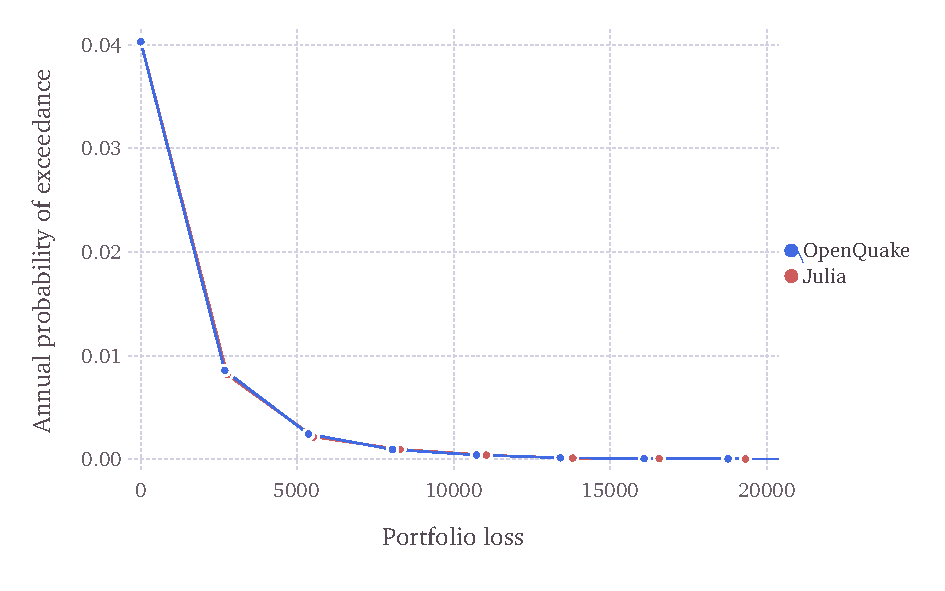
\includegraphics[width=12cm]{qareport/figures/fig-lc-ebr-6b}
\caption{Portfolio loss curve comparison for event based risk test case 6b}
\label{fig:lc-ebr-6b}
\end{figure}